\chapter{Classic Provenance}
\label{chap:classic_provenance}

\section{What is Provenance?}

\subsection{Definition}
% Dictionary entry
Provenance - \textit{source, origin} \cite{prov_dict}. 
% General explanation
In computing, provenance information describes the origins and the history of data within its lifetime. When talking about database management systems, the commonly used term is \textit{data provenance} \cite{cheney2009provenance}. The idea behind data provenance is keeping additional information (meta-data) allowing us to easily answer a large number of ``meta-questions".
% Provenance as explanations for query results
\par Data provenance helps with providing explanations for the existence of tuples in a query result. The context of these explanations is the DB state prior to the query execution. \\

% Intro to notions of data provenance
\subsection{Related Work} Over the past 15 years, provenance research has advanced in addressing both theoretical \cite{cheney2009provenance, green2007provenance, Deutch2014} 
and practical \cite{Ives2008, Karvounarakis2010, Deutch2015, Deutch2017, Senellart2018, DBLP:conf/cidr/IvesZHZ19} 
aspects. 
In particular, several different notions of data provenance (\textit{lineage}, \textit{why}, \textit{how} and \textit{where}) were formally defined \cite{Cui:2000:TLV:357775.357777, DBLP:conf/icdt/BunemanKT01,  cheney2009provenance}.
% Related Work - Provenance Approximation and Summarization
\par A few prior works \cite{approx_lineage, approx_PROX, approx_summary, approx_why_and_why_not} focus on approximate (or summarized) provenance. That is, seeking a compact representation of the provenance at the possible cost of information loss in an attempt to deal with the growing size and complexity of exact provenance information in real-life systems.


\section{Provenance Semirings}\label{sec:semiring provenance}
% Overview and definition - Val Tannen and T.J. Green
\subsection{Overview}\footnotemark
\footnotetext{Portions of this section were adapted from Green et al. \cite{green2007provenance} and Karvounarakis et al. \cite{Karvounarakis:2012:SDQ:2380776.2380778}.}
\textit{Provenance semirings} have been introduced by Green et al. \cite{green2007provenance} as a formalism for data provenance. These semirings have been shown \cite{Karvounarakis:2012:SDQ:2380776.2380778} to generalize previous works such as lineage \cite{Cui:2000:TLV:357775.357777} and why-provenance \cite{DBLP:conf/icdt/BunemanKT01}. The main idea is based on annotating every tuple in the DB with elements from some algebraic structure $(K,+,\cdot,0,1)$\footnotemark
\footnotetext{$K$ is a set, containing two distinguished elements $0,1$; and $+,\cdot$ are binary operators on elements from $K$.}
resulting in \textit{K-relations}\footnotemark, 
\footnotetext{Informally, relations in which tuples are annotated with elements from $K$.}
and extending $\mathcal{RA^+}$ (relational algebra, excluding the difference operator) to operate on $K$-relations via definitions in terms of the abstract + and $\cdot$ operations of $K$:
\begin{itemize}
    \item + corresponds to alternative use of data (union - $\cup$ or projection - $\Pi$);
    \item $\cdot$ corresponds to joint use of data (join - $\bowtie$);
    \item $0$ and $1$ are used for selection ($\sigma$) predicates.
\end{itemize}
Note, this method has to comply with common $\mathcal{RA^+}$ identities in order to correctly extend to $K$-relations:
\begin{itemize}
    \item join and union are both associative and commutative;
    \item union has identity $\emptyset$;
    \item join is distributive over union;
    \item $\sigma_{false}(R) = \emptyset$ and $\sigma_{true}(R) = R$.
\end{itemize}
Green et al. \cite{green2007provenance} showed that these identities hold for $\mathcal{RA^+}$ on $K$-relations \textit{iff} $(K,+,\cdot,0,1)$ is a \textit{commutative semiring}.
I.e., $(K,+,0)$ and $(K,\cdot,1)$ are commutative monoids\footnotemark,
\footnotetext{An algebraic structure that is closed under an associative binary operation and has an identity element.} 
$\cdot$ is distributive over + and $\forall a, 0 \cdot a = a \cdot 0 = 0$. \\

% Important Cases
\subsection{Important cases} Several important semirings that are discussed in the literature \cite{green2007provenance, Karvounarakis:2012:SDQ:2380776.2380778, Senellart2017} are:
\begin{itemize}
    \item $(\mathbb{B}, \vee, \wedge, false, true)$ - binary trust (set semantics);
    \item $(\mathbb{N}, +, \cdot, 0, 1)$ - multiplicity (bag semantics);
    \item $(\mathbb{A}, min, max, 0, P)$ - security semiring (access control), where the total order $\mathbb{A}=P<C<S<T<0$ describes levels of security clearance: $P$ public, $C$ confidential, $S$ secret, and $T$ top-secret;
    \item $([0,1], max, \cdot, 0, 1)$ - Viterbi semiring (confidence scores, probability);
    % \item $(\mathbb{N}\cup\{\infty\}, min, +, \infty, 0)$ - tropical semiring (data pricing);
    \item $(\mathbb{N}[X], 0, 1, +, \cdot)$ - used for a general form of provenance, the provenance polynomials (the universal semiring). $\mathbb{N}[X]$ is the set of multivariate polynomials with coefficients from $\mathbb{N}$ and variables from a set $X$.
\end{itemize}

\section{ProvSQL - A Real World Provenance Application}\label{sec:provsql}
% Goal
ProvSQL is an open-source project developed by Pierre Senellart et al. \cite{Senellart2018}.
According to the official GitHub page \cite{provsql_github}:
``The goal of the ProvSQL project is to add support for (m-)semiring provenance and uncertainty management to PostgreSQL databases, in the form of a PostgreSQL extension/module/plugin. It is work in progress at the moment." \\
Next, we present several concepts that are incorporated in ProvSQL and briefly discuss its implementation.
% m-semirings
\subsection{Semirings with monus} We previously stated in section \ref{sec:semiring provenance} that provenance semirings extend only to  $\mathcal{RA^+}$ queries. However, \cite{monus_k_relations} identified a large class of semirings that (subject to certain restrictions) can be equipped with a monus operator $-$. Thus, it is possible to generalize provenance capturing to $\mathcal{RA}$ with a difference $(\setminus)$ operation (adding support for non-monotone\footnotemark queries). 
\footnotetext{$I \subseteq I' \notimplies Q(I) \subseteq Q(I')$.}
This class of semirings is called \textit{m-semirings}. Furthermore, \cite{monus_k_relations} show a universal m-semiring, i.e., it is possible to obtain a provenance evaluation in any other m-semiring by applying the appropriate semiring homomorphism.
% Provenance Circuits
\subsection{Provenance Circuits}\label{sec:provenance circuits}
As shown previously by Green et al. \cite{green2007provenance} and Karvounarakis et al. \cite{Karvounarakis:2012:SDQ:2380776.2380778}, provenance explanations can be expressed via semiring formulas (polynomials). These formulas may blow-up in terms of space consumption, and, thus, they are problematic for practical use. An alternative (more compact) representation for provenance annotations is  \textit{circuits} \cite{Deutch2014, Senellart2017}, which are constructed per-query. A provenance circuit is an inductively built directed acyclic graph (DAG), with the following properties:
\begin{itemize}
    \item The leaves contain annotations of tuples from the input DB.
    \item Inner nodes represent operators from a particular semiring (termed \textit{gates} by Senellart et al.). 
    \item The edges (termed \textit{wires} by Senellart et al.) connect nodes to an operator, representing an intermediate calculation.
    \item The sub-DAG under a given node represents the semiring formula for deriving it. 
\end{itemize}
% PostgreSQL Hooks
\subsection{PostgreSQL Hooks} PostgreSQL (Postgres) hooks \cite{postgre_hooks} make it possible to extend/modify its behaviour without rebuilding Postgres, by interrupting the execution process at certain points. Similarly to Postgres itself, the hooks API is written in C. Every hook is accessible via a global function pointer, initially set to \texttt{NULL}. During an extension's loading (following a \texttt{CREATE EXTENSION} command) Postgres calls the extension's own \texttt{\_PG\_init} function (if implemented), which has access to the hooks handler pointers (at this point, a hook function can be registered). When Postgres needs to call a hook, it checks the relevant function pointer, and calls the registered function, if the pointer is set.
% Implementation
\usetikzlibrary{calc,trees,positioning,arrows,chains,shapes.geometric,%
    decorations.pathreplacing,decorations.pathmorphing,shapes,%
    matrix,shapes.symbols}

\tikzset{
>=stealth',
  punktchain/.style={
    rectangle, 
    rounded corners, 
    % fill=black!10,
    draw=black, very thick,
    text width=22em, 
    minimum height=3em, 
    text centered, 
    on chain},
  line/.style={draw, thick, <-},
  element/.style={
    tape,
    top color=white,
    bottom color=blue!50!black!60!,
    minimum width=8em,
    draw=blue!40!black!90, very thick,
    text width=10em, 
    minimum height=3.5em, 
    text centered, 
    on chain},
  every join/.style={->, thick,shorten >=1pt},
  decoration={brace},
  tuborg/.style={decorate},
  tubnode/.style={midway, right=2pt},
}
\begin{figure}[htb]
\small
  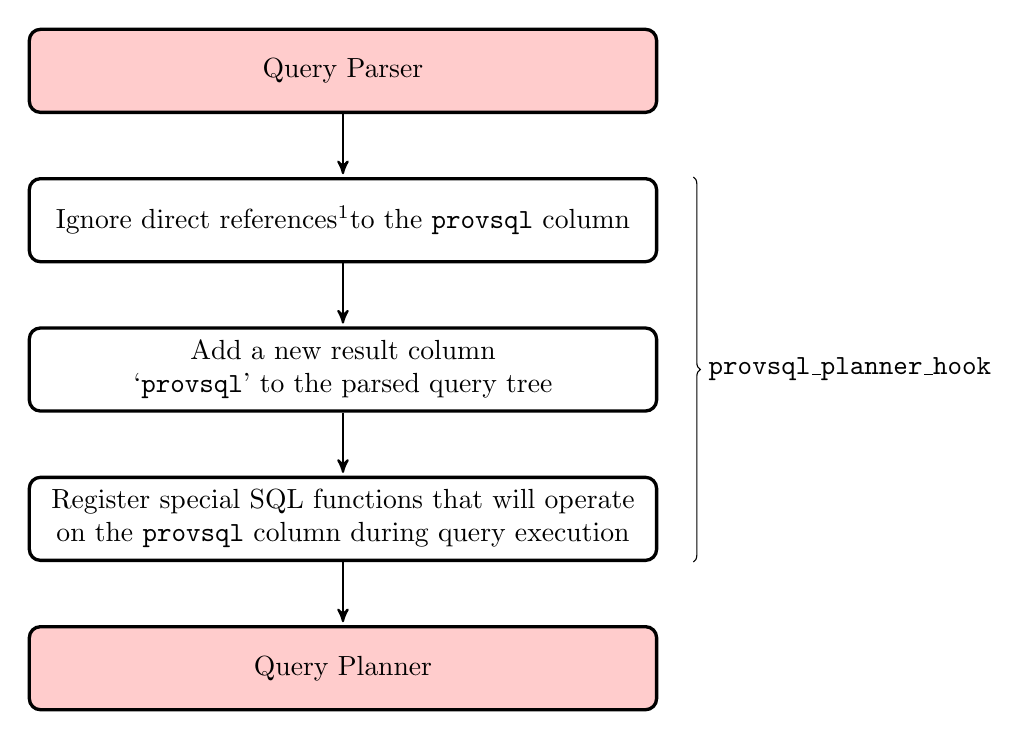
\begin{tikzpicture}
  [node distance=.8cm,
  start chain=going below,]
    %  \node[punktchain, fill=yellow!20] (input) {Input query};
     \node[punktchain, join, fill=red!20] (parser) {Query Parser};
     \node[punktchain, join] (A) {Ignore direct references\footnotemark to the \texttt{provsql} column};
     \node[punktchain, join] (B) {Add a new result column `\texttt{provsql}' to the parsed query tree};
     \node[punktchain, join] (C) {Register special SQL functions that will operate on the \texttt{provsql} column during query execution};
    \node[punktchain, join, fill=red!20] (planner) {Query Planner};
    % \node[punktchain, join, fill=green!20] (output) {Query result:\\ includes a \texttt{provsql} column of tokens, identifying gates of the prov. circuit};
  % Now that we have finished the main figure let us add some "after-drawings"
  % Now, let us add some braches. 
  %% No. 1
%   \draw[tuborg, decoration={brace}] let \p1=(init.north), \p2=(init.south) in
%     ($(2, \y1)$) -- ($(2, \y2)$) node[tubnode] {Called once, upon extension loading};
%   %% No. 2
%   \draw[tuborg, decoration={brace}] let \p1=(fini.north), \p2=(fini.south) in
%     ($(2, \y1)$) -- ($(2, \y2)$) node[tubnode] {Called once, upon extension unloading};
  %% No. 3
  \draw[tuborg, decoration={brace}] let \p1=(A.north), \p2=(C.south) in
    ($(4.45, \y1)$) -- ($(4.45, \y2)$) node[tubnode] {\texttt{provsql\_planner\_hook}};
  \end{tikzpicture}
   \textbf{\caption{\label{fig:provsql_architecture}ProvSQL system architecture.\\
   The red rectangles are a part of Postgres's built in execution pipeline. The white rectangles are ProvSQL's implementation of a \texttt{planner\_hook}, which we use for the provenance-related calculations.}}
\normalsize
\end{figure}
\footnotetext{Explicit mentions of the \texttt{provsql} column in the query (in any of the \texttt{SELECT}, \texttt{FROM} or \texttt{WHERE} clauses).}
%%% Local Variables: 
%%% mode: latex
%%% TeX-master: t
%%% End:
\subsection{Implementation} ProvSQL \cite{provsql_github} uses the \texttt{planner\_hook}, which is called after a query has been parsed, and before it is sent to the query planner. The system architecture (as part of Postgres's query execution pipeline) is depicted in Figure \ref{fig:provsql_architecture}.
ProvSQL currently supports a wide range of non-aggregate SQL queries (for more details see \cite{provsql_github, Senellart2018}). The generated query result includes a \texttt{provsql} column of unique\footnotemark
\footnotetext{128-bit universally unique identifiers (UUIDs) that are generated using the \texttt{uuid-ossp} PostgreSQL module.}
tokens, identifying gates of the provenance circuit.

